\begin{frame}
	\frametitle{Die Klasse $\PH$}
	\framesubtitle{Definition von $\PH$}
	
	\begin{KITinfoblock}{Definition	$\sum_{i}^{p} $ }
		$\sum_{i}^{p} $ ist die Menge aller Sprachen L f\"ur die gilt : \newline
		Es gibt deterministische polynomielle TM $M$ und ein Polynom $q$ so, dass :
		\newline
		
		$x \in L \Leftrightarrow \exists u_1 \in {\lbrace 0,1 \rbrace }^{q(|x|)}$
		$\forall u_2 \in {\lbrace 0,1 \rbrace }^{q(|x|)}$
		$\ldots \mathcal{Q}_i u_i \in {\lbrace 0,1 \rbrace }^{q(|x|)}$
		$M(x,u_1 ,\ldots , u_i) = 1$	\newline
		
		gilt,wobei $\mathcal{Q}_i$ entweder $\forall$ oder $\exists$ beschreibt,
		abh\"angig davon ob $i$ gerade oder ungerade ist.
	\end{KITinfoblock}
	\pause
	\bigskip
	
	\begin{KITinfoblock}{Definition $\PH$}
		Die polynomielle Hierarchie ist $\PH = {\cup}_{i \in \mathbb{N}} \sum_{i}^{p}$
	\end{KITinfoblock}
\end{frame}
\begin{frame}
	\begin{columns}
	\column{.5\textwidth}
	\begin{overprint}
	\only<1>{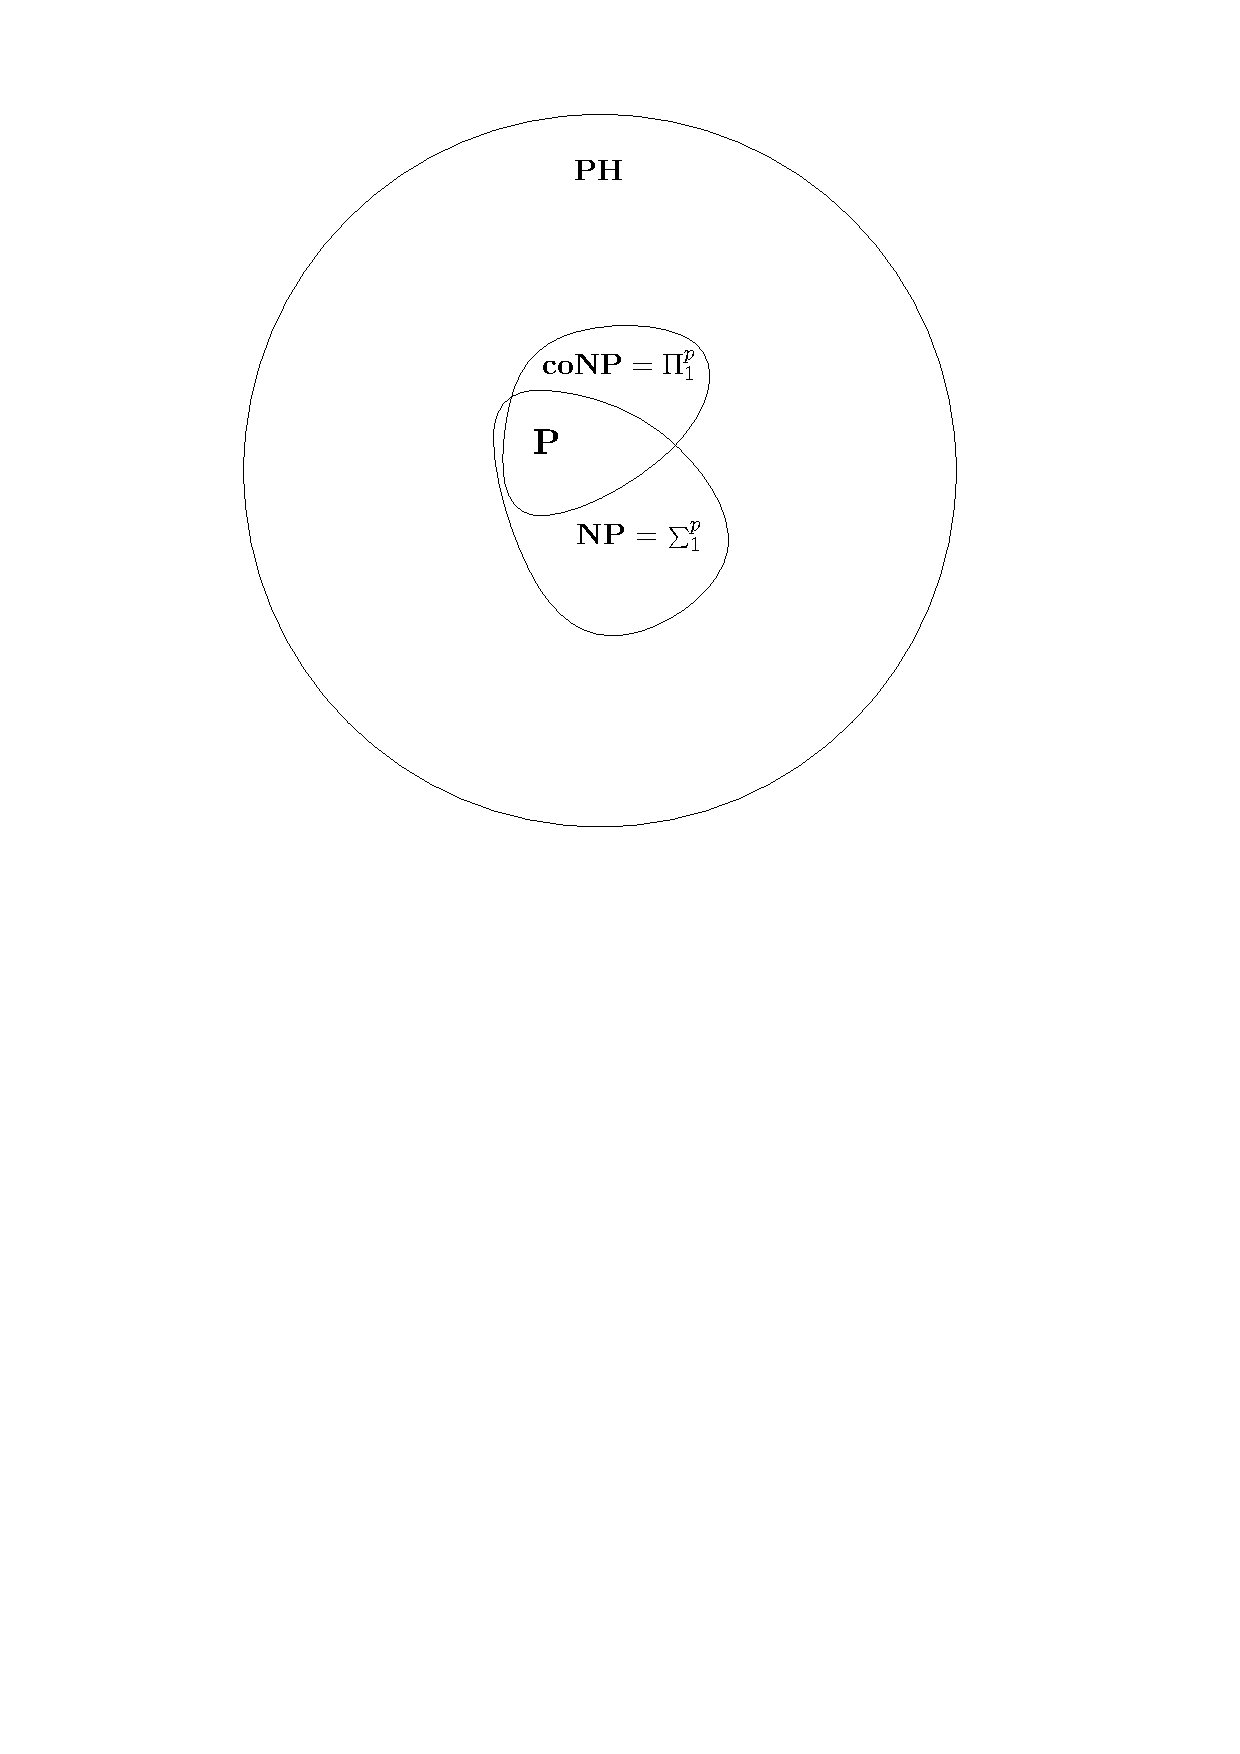
\includegraphics[page=1, scale= 0.5]{images/polyhierarchy2.pdf}}
	\only<2>{\includegraphics[page=2, scale= 0.5]{images/polyhierarchy2.pdf}}
	\only<3>{\includegraphics[page=3, scale= 0.5]{images/polyhierarchy2.pdf}}
	\only<4>{\includegraphics[page=4, scale= 0.5]{images/polyhierarchy2.pdf}}
	\end{overprint}
	\column{.5\textwidth}
	\begin{itemize}
		  \item Man sieht : $\sum_{1}^{p} = \NP$
		  \item $\Pi_{i}^{p} := co\sum_{i}^{p}$
		  \item $\sum_{i}^{p} \subseteq \Pi_{i+1}^{p} \subseteq \sum_{i+2}^{p}$
		\end{itemize}
	\end{columns}
\end{frame}
\begin{frame} 
	\frametitle{Die Klasse $\PH$}
	\framesubtitle{Eigenschaften von $\PH$}
	
	\begin{itemize}[<+->]
		\item Vermutung: $\P \neq \NP$ und $\NP \neq \coNP$	
		\item Verallgemeinerung:    $\sum_{i}^{p}  \subsetneq \sum_{i+1}^{p}$ für alle $i$
		\item "The polynomial hierarchy does not collapse"
	\end{itemize}
	\bigskip
	\pause
	\begin{KITinfoblock}{Satz: Kollaps von $\PH$ und Auswirkungen auf $\P-\NP$}
		\begin{enumerate}[<+->]
			\item Für alle $ i \geq 0$ gilt: $ \quad \sum_{i}^{p} = \prod_{i}^{p} \quad \Rightarrow \quad \PH = \sum_{i}^{p}$
			\item Wenn $\P = \NP$, dann folgt $\PH = \P$
		\end{enumerate}
	\end{KITinfoblock}
\end{frame}
\begin{frame} 
	\frametitle{Die Klasse $\PH$}
	\framesubtitle{Beweis}
	\heading{Beweis von $ \P = \NP \Rightarrow \PH = \P$}
	\begin{itemize}[<+->]
		\item Sei $\P = \NP$, beweisen über Induktion $\sum_{i}^{p},\prod_{i}^{p} \subseteq \P$ für alle $i$
		\bigskip
		\item \galert{IA}: $i=1$, nach Voraussetzung: $\sum_{1}^{p} = \NP$,\quad$\prod_{1}^{p} = \coNP$ \newline
				und $\P = \co\P = \NP = \coNP$ gilt
		\bigskip
		\item \galert{IV}: Es gelte  $\sum_{i-1}^{p} \subseteq \P$ für $i-1 \in \mathbb{N}$  
		\item Anm: $\prod_{i-1}^{p}$ besteht aus Komplementsprachen der Sprachen in $\sum_{i-1}^{p}$ \newline $\P$ ist abgeschlossen unter Komplementbildung $\Rightarrow$  $\prod_{i-1}^{p} \subseteq \P$ unter IV.
		
	 
		
	\end{itemize}
\end{frame} 

	
\begin{frame}
	\frametitle{Die Klasse $\PH$}
	\framesubtitle{Beweis}
	\begin{itemize}[<+->]
		\item \galert{IS}: Sei $L \in \sum_{i}^{p}$, dann ex. TM $M$ und Polynom $q$ so, dass \newline
		\begin{align}
			x \in L \Leftrightarrow  \exists u_1 \in \{0,1\}^{q(|x|)} &\forall u_2  \in \{0,1\}^{q(|x|)} ... \ \mathcal{Q}_i u_i \in \{0,1\}^{q(|x|)}  \notag \\
			&M(x,u_1,u_2,...,u_i)=1 \notag
		\end{align}
		gilt
		\bigskip
		\item Definiere Sprache $L'$
		\begin{align}
		(x,u_1) \in L' \Leftrightarrow \forall u_2 \in &\{0,1\}^{q(|x|)} ... \ \mathcal{Q}_i u_i \in \{0,1\}^{q(|x|)} \notag \\ &M(x,u_1,u_2, ... u_i) = 1 \notag 
		\end{align}
	
	\end{itemize}
\end{frame}
\begin{frame}
	\frametitle{Die Klasse $\PH$}
	\framesubtitle{Beweis}
		\begin{itemize}[<+->]
				\item $L'$ ist in $\prod_{i-1}^{p}$, denn
				\begin{align}
					(x,u_1) \in L' \Leftrightarrow \forall u_2 \in &\{0,1\}^{q(|x|)} ... \ \mathcal{Q}_i u_i \in \{0,1\}^{q(|x|)} \notag \\ &M(x,u_1,u_2, ... u_i) = 1 \notag 
				\end{align}
				\begin{align}
					(x,u_1) \in \overline{L'} \Leftrightarrow \exists u_2 \in &\{0,1\}^{q(|x|)} ... \ \mathcal{Q}_i u_i \in \{0,1\}^{q(|x|)} \notag \\ &\overline{M(x,u_1,u_2, ... u_i)} = 1 \notag 
				\end{align}
				\item Also $\overline{L'} \in \sum_{i-1}^{p}$ und damit folgt Behauptung.
		\end{itemize}
\end{frame}
\begin{frame}
	\frametitle{Die Klasse $\PH$}
	\framesubtitle{Beweis}
		\begin{itemize}[<+->]
			\item $L'$ ist in $\prod_{i-1}^{p}$ 
			\item Nach IV gilt: $ \quad \prod_{i-1}^{p} \in \P  \quad \Rightarrow \quad L' \in \P$
			\item Damit ex. det. TM $M'$, die $L'$ in polynom. Zeit berechnet
			\item Nach Konstruktion gilt: $x \in L \Leftrightarrow \exists u_1 \in \{0,1\}^{q(|x|)} (x,u_1) \in L'$
			\item  \[x \in L \Leftrightarrow \exists u_1 \in \{0,1\}^{q(|x|)} M'(x,u_1) = 1 \] 
			\item Damit $L \in \NP$ und da $\P = \NP$ vorausgesetzt, folgt $L \in \P$
			\item Somit  $\sum_{i}^{p},\prod_{i}^{p} \subseteq \P$ für alle $i$
			\item Also $\PH = \P$
			\qed
	\end{itemize}
\end{frame}
\begin{frame}
	\frametitle{Die Klasse $\PH$}
	\framesubtitle{$\PH$ Vollst\"andigkeit}
	
	Wir definieren $\PH$ Vollst\"andigkeit analog zur $\NP$ Vollständigkeit und
	erhalten damit :
	\pause
	\bigskip
	
	\begin{KITinfoblock}{Überlegung zur $\PH$ Vollst\"andigkeit}
		Wenn eine $\PH$-vollst\"andige Sprache L existiert dann existiert ein $i$
		so, dass $\PH = \sum_{i}^{p}$
	\end{KITinfoblock}
	\bigskip
	\pause
	Beweis :
	\begin{itemize}[<+->]
	  \item Da $\PH = \cup_{k \in \mathbb{N}} \sum_{k}^{p}$   $\exists i$ so dass
	  $L \in \sum_{i}^{p}$
	  \item K\"onnen durch $\PH$ Vollständigkeit jedes $L' \in \PH$ in pol. Zeit
	  auf L reduzieren
	  \item und damit also auch $L' \in \sum_{i}^{p}$	\qed
	\end{itemize}
	
\end{frame}